\documentclass[tikz,border=5pt]{standalone}
\usepackage{pgfplots}
\pgfplotsset{compat=1.18}
\begin{document}
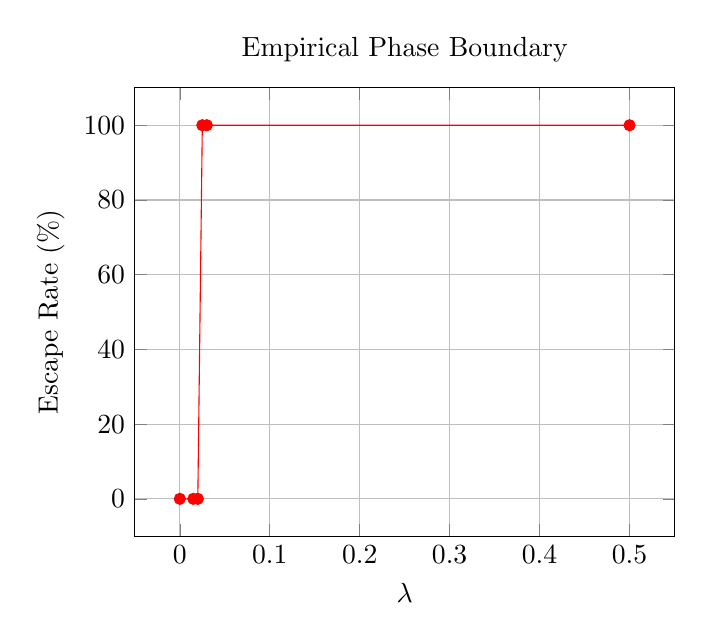
\begin{tikzpicture}
\begin{axis}[
    title={Empirical Phase Boundary},
    xlabel={$\lambda$},
    ylabel={Escape Rate (\%)},
    grid=major
]
\addplot[red, mark=*] coordinates {(0.0,0) (0.015,0) (0.02,0) (0.025,100) (0.03,100) (0.5,100)};
\end{axis}
\end{tikzpicture}
\end{document}
